\documentclass[letterpaper]{article}
\usepackage[margin=1in]{geometry}
\usepackage[utf8]{inputenc}
\usepackage{textcomp}
\usepackage{amssymb}
\usepackage{natbib}
\usepackage{graphicx}
\usepackage{gensymb}
\usepackage{amsthm, amsmath, mathtools}
\usepackage[dvipsnames]{xcolor}
\usepackage{enumerate}
\usepackage{mdframed}
\usepackage[most]{tcolorbox}
\usepackage{csquotes}
% https://tex.stackexchange.com/questions/13506/how-to-continue-the-framed-text-box-on-multiple-pages

\tcbuselibrary{theorems}

\newcommand{\R}{\mathbb{R}}
\newcommand{\Z}{\mathbb{Z}}
\newcommand{\N}{\mathbb{N}}
\newcommand{\Q}{\mathbb{Q}}
\newcommand{\C}{\mathbb{C}}
\newcommand{\code}[1]{\texttt{#1}}
\newcommand{\mdiamond}{$\diamondsuit$}
\newcommand{\PowerSet}{\mathcal{P}}
\newcommand{\Mod}[1]{\ (\mathrm{mod}\ #1)}
\DeclareMathOperator{\lcm}{lcm}

%\newtheorem*{theorem}{Theorem}
%\newtheorem*{definition}{Definition}
%\newtheorem*{corollary}{Corollary}
%\newtheorem*{lemma}{Lemma}
\newtheorem*{proposition}{Proposition}


\newtcbtheorem[number within=section]{theorem}{Theorem}
{colback=green!5,colframe=green!35!black,fonttitle=\bfseries}{th}

\newtcbtheorem[number within=section]{definition}{Definition}
{colback=blue!5,colframe=blue!35!black,fonttitle=\bfseries}{def}

\newtcbtheorem[number within=section]{corollary}{Corollary}
{colback=yellow!5,colframe=yellow!35!black,fonttitle=\bfseries}{cor}

\newtcbtheorem[number within=section]{lemma}{Lemma}
{colback=red!5,colframe=red!35!black,fonttitle=\bfseries}{lem}

\newtcbtheorem[number within=section]{example}{Example}
{colback=white!5,colframe=white!35!black,fonttitle=\bfseries}{def}

\newtcbtheorem[number within=section]{note}{Important Note}{
        enhanced,
        sharp corners,
        attach boxed title to top left={
            xshift=-1mm,
            yshift=-5mm,
            yshifttext=-1mm
        },
        top=1.5em,
        colback=white,
        colframe=black,
        fonttitle=\bfseries,
        boxed title style={
            sharp corners,
            size=small,
            colback=red!75!black,
            colframe=red!75!black,
        } 
    }{impnote}
\usepackage[utf8]{inputenc}
\usepackage[english]{babel}
\usepackage{fancyhdr}
\usepackage[hidelinks]{hyperref}

\pagestyle{fancy}
\fancyhf{}
\rhead{CSE 101}
\chead{Monday, January 24, 2022}
\lhead{Lecture 8}
\rfoot{\thepage}

\setlength{\parindent}{0pt}

\begin{document}

\section{Priority Queue Implementations}
The implementation of Dijkstra's algorithm is very much dependent on the priority queue that we use. That is, depending on how we implement our priority queue, we may or may not see a change in performance. So, we will go through some prioriy queue implementations. 

\subsection{Unsorted List}
Store $n$ elements in an unsorted list. 

\begin{center}
    \begin{tabular}{p{0.85in}|p{0.75in}|p{4.4in}}
        \textbf{Operation} & \textbf{Runtime} & \textbf{Explanation} \\ 
        \hline 
        \code{Insert}      & $\BigO(1)$ & Add it at the end of the list. \\ 
        \code{DecreaseKey} & $\BigO(1)$ & Assuming the operation comes with a pointer to where the element is stored in your data structure, take that element and decrease its key value. \\ 
        \code{DecreaseMin} & $\BigO(n)$ & We need to potentially scan the entire list. \\ 
    \end{tabular}
\end{center}
For Dijkstra, we would have $\BigO(|V|^2 + |E|)$. 

\subsection{Binary Heap}
Store elements in a balanced binary tree with each element having smaller key value than its children.

\begin{center}
    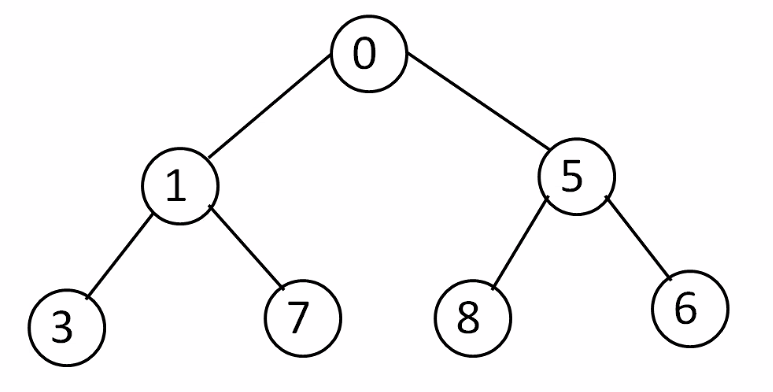
\includegraphics[scale=0.5]{../assets/bin_heap.png}

    \textbf{Figure:} A binary heap.
\end{center}
The smallest key is at the top (\code{0}) and there are $\log{n}$ levels. 

\begin{center}
    \begin{tabular}{p{0.85in}|p{0.75in}|p{4.4in}}
        \textbf{Operation} & \textbf{Runtime} & \textbf{Explanation} \\ 
        \hline 
        \code{Insert}      & $\BigO(\log(n))$ & Add the key at the bottom, then bubble the new key up until it's in the right place. \\ 
        \code{DecreaseKey} & $\BigO(\log(n))$ & We need to change the key. Then, we might need to bubble up the changed key until it's in the right place. \\ 
        \code{DecreaseMin} & $\BigO(\log(n))$ & We remove and then return the root node. Then, we move the bottom-most node to the root. After this, we might need to continuously bubble down the root node until it's in the right place. \\ 
    \end{tabular}
\end{center}
For Dijkstra, we would have $\BigO(\log(|V|)(|V| + |E|))$. 


\subsection{d-ary Heap}
This is like a binary heap, but each node has $d$ children. 
\begin{center}
    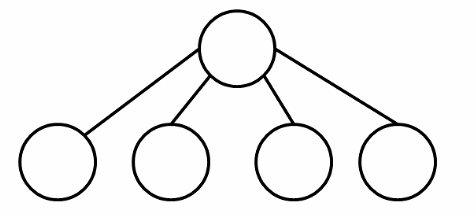
\includegraphics[scale=0.5]{../assets/dary_heap.png}

    \textbf{Figure:} A 4-ary heap.
\end{center}

There are $\frac{\log(n)}{\log(d)}$ levels, so bubble up is faster. However, bubble down is slower since we need to compare more children. 

\begin{center}
    \begin{tabular}{p{0.85in}|p{0.75in}|p{4.4in}}
        \textbf{Operation} & \textbf{Runtime} & \textbf{Explanation} \\ 
        \hline 
        \code{Insert}      & $\BigO\left(\frac{\log(n)}{\log(d)}\right)$ & Same thing as binary heap, essentially. \\ 
        \code{DecreaseKey} & $\BigO\left(\frac{\log(n)}{\log(d)}\right)$ & Same idea as binary heap, \emph{but} the bubbling up is a lot faster. \\ 
        \code{DecreaseMin} & $\BigO\left(\frac{d\log(n)}{\log(d)}\right)$ & This is because, for bubble down, we need to compare more children; specifically, the $d$ children. \\ 
    \end{tabular}
\end{center}
For Dijkstra, we would have $\BigO\left(\frac{\log(|V|)(d|V| +|E|)}{\log(d)}\right)$. If the number of edges is substantially greater than the number of vertices, this can potentially be an improvement. 


\subsection{Fibonacci Heap}
This is an advanced data structure that uses amortization\footnote{So, you might spend more time on a particular operation, but the overall runtime will be ``consistent.''}. We are not concerned with its implementation. 

\begin{center}
    \begin{tabular}{p{0.85in}|p{0.75in}}
        \textbf{Operation} & \textbf{Runtime} \\ 
        \hline 
        \code{Insert}      & $\BigO(1)$ \\ 
        \code{DecreaseKey} & $\BigO(1)$ \\ 
        \code{DecreaseMin} & $\BigO(\log(n))$ \\ 
    \end{tabular}
\end{center}
For Dijkstra, we would have $\BigO(|V|\log(|V|) + |E|)$. This is the most ideal runtime, and thus the runtime that we can assume. 




\newpage 
\section{Negative Edge Weights}
So far, we've talked about non-negative lengths. However, depending on what we're representing as lengths, we might have \emph{negative} lengths. That being said, the problem statement is the same - find the path with the smallest sum of edge weight. 

\bigskip 

Right now, Dijkstra's algorithm doesn't actually work on negative edge values. To see why this is the case, consider the following visualization: 
\begin{center}
    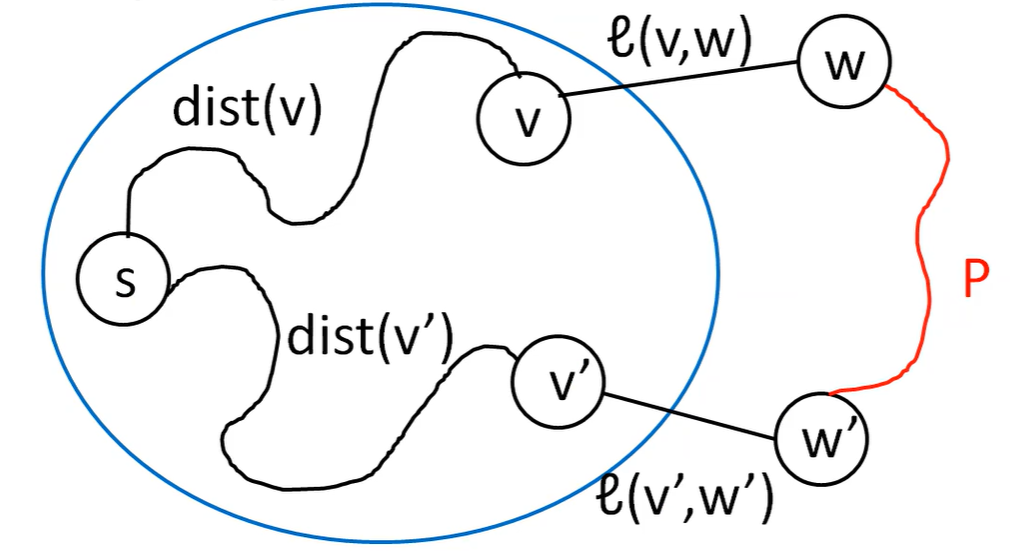
\includegraphics[scale=0.3]{../assets/neg_bubble.png}
\end{center}
Here, the bubble represents all correctly assigned distances. In other words, here, $s$ and and $v$ has edge length $\text{dist}(v)$, the shortest distance between the two. Then, from $v$ (inside the bubble) to $w$ (outside the bubble), if we consider the edge length $\ell(v, w)$, it follows that this must be the shortest path. The point was that this must be the right distance to $w$; any other way to get to $w$ means that we would have to leave the bubble some other way (in our case, from $s$ to $v'$ to $w'$). Then, there has to be a path connecting $w'$ to $w$, of which we denote $P$. So, it follows that:  
\[\text{dist}(v) + \ell(v, w) \leq \text{dist}(v') + \ell(v', w') + \ell(P)\]
This correctly works if $\ell(P)$ is non-negative. However, if $\ell(P)$ is negative, we run into an issue. 

\subsection{Negative Weight Cycle}
\begin{definition}{}{}
    A \textbf{negative weight cycle} is a cycle where the total weight of edges is negative. 
\end{definition}
\textbf{Remarks:}
\begin{itemize}
    \item If $G$ has a negative weight cycle, then there are probably no shortest paths since we can go around the cycle over and over again. 
    \item For an undirected graph $G$, a single negative weight edge gives a negative weight cycle by going back and forth on it. So, we usually don't talk about the negative edge weight in the context of an undirected graph. 
\end{itemize}
For example, consider the following graph:
\begin{center}
    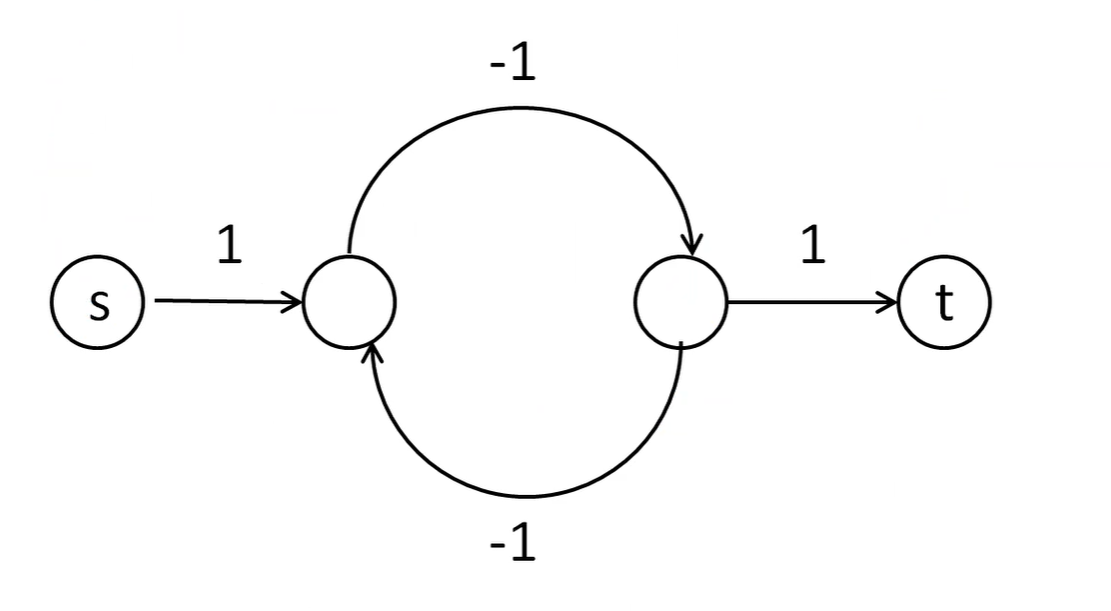
\includegraphics[scale=0.2]{../assets/neg_cycle_1.png}
\end{center}
Here, the shortest path length from $s$ to $t$ is as small as we like it to be. So, really, the shortest path length is $-\infty$. This graph\textbf{also} answers an important question:
\begin{mdframed}[]
    What stops us from adding a constant to every edge length so every edge length is non-negative, thus letting us run Dijkstra's algorithm? 
\end{mdframed}
Well, if we added a constant to every edge length so that every edge length is non-negative, then there would only be one answer. For example, if we added 1 to each edge length, the shortest path becomes $2 + 0 + 2 = 4$. But since we added 1 to each edge length and we went through three edges, our final answer is $1$. \emph{However}, this completely avoids the fact that we could just loop around the negative cycle many times. 

\end{document}